\documentclass{article}

\usepackage{tikz}
\usepackage{tikz}
\usepackage{pgfplots}
\usetikzlibrary{backgrounds, positioning, fit}
\usetikzlibrary{shapes.geometric}
\usetikzlibrary{patterns}
\usepackage[T1]{fontenc}
%% put tikzlibrary below if necessary

% set up externalization
\usetikzlibrary{external}
\tikzset{external/system call={latex \tikzexternalcheckshellescape -halt-on-error
-interaction=batchmode -jobname "\image" "\texsource";
dvips -o "\image".ps "\image".dvi;
ps2eps "\image.ps"}}
\tikzexternalize

\tikzstyle{nd} = [circle,fill,draw,text=white,font=\sffamily,minimum size=2mm]
\tikzstyle{input} = [rectangle, rounded corners, minimum width=2cm, minimum height=1cm,text centered, draw=black, fill=gray!15]
\tikzstyle{record} = [rectangle, rounded corners, minimum width=2cm, minimum height=0.3cm,text centered, draw=black]

\tikzstyle{layer1} = [rectangle, rounded corners, minimum width=0.25cm, minimum height=3cm,text centered, draw=black, fill=gray!15]
\tikzstyle{layer2} = [rectangle, rounded corners, minimum width=0.25cm, minimum height=2cm,text centered, draw=black, fill=gray!15]
\tikzstyle{latent} = [circle, text centered, draw=black, inner sep=0pt, minimum size=2cm, fill= gray!20]


\tikzstyle{layer11} = [rectangle, rounded corners, minimum width=0.25cm, minimum height=3cm,text centered, draw=black, fill=gray!15]
\tikzstyle{layer12} = [rectangle, rounded corners, minimum width=0.25cm, minimum height=2cm,text centered, draw=black, fill=gray!15]
\tikzstyle{layer13} = [rectangle, rounded corners, minimum width=0.25cm, minimum height=1.5cm,text centered, draw=black, fill=gray!15]
\tikzstyle{layer14} = [rectangle, rounded corners, minimum width=0.25cm, minimum height=1cm,text centered, draw=black, fill=gray!15]


\begin{document}

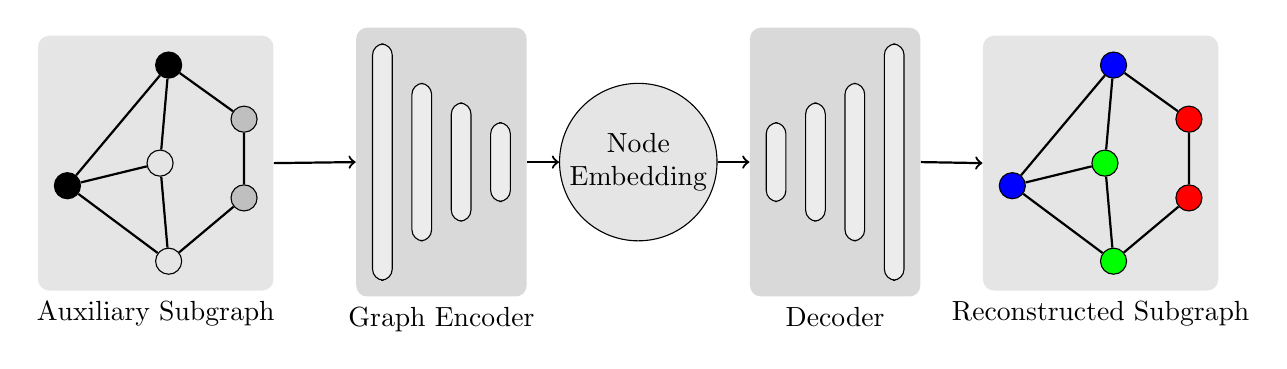
\begin{tikzpicture}

\path node[fill=black,nd,xshift=-8cm,yshift=-0.3cm] (1) {} -- ++ (50:2) node[fill=black,nd,xshift=-8cm,yshift=-0.3cm] (2) {} -- ++(-95:1.25) node[fill=gray!20,nd,xshift=-8cm,yshift=-0.3cm] (3) {} -- ++(-85:1.25) node[fill=gray!20,nd,xshift=-8cm,yshift=-0.3cm] (4) {} -- ++(40:1.25) node[fill=gray!50,nd,xshift=-8cm,yshift=-0.3cm] (5) {} -- ++ (0,1) node[fill=gray!50,nd,xshift=-8cm,yshift=-0.3cm] (6) {} ;
\draw[thick] (1)--(2)--(6)--(5)--(4)--(1)--(3)--(2)--(3)--(4);

\begin{scope}[on background layer]
     \node (target) [fit=(1) (2) (3) (4) (5) (6), fill= gray!20, rounded corners, inner sep=.2cm, label={below:Auxiliary Subgraph}] {};
\end{scope}


\node (en1) [layer11]  at (-4,0) {};
\node (en2) [layer12]  at (-3.5,0) {};
\node (en3) [layer13]  at (-3,0) {};
\node (en4) [layer14]  at (-2.5,0) {};


\node (dec1) [layer14]  at (1,0) {};
\node (dec2) [layer13]  at (1.5,0) {};
\node (dec3) [layer12]  at (2,0) {};
\node (dec4) [layer11]  at (2.5,0) {};


\node (latent) [latent,align=center] at (-0.75,0) {Node\\ Embedding};

\begin{scope}[on background layer]
    \node (encoder) [fit=(en1) (en2) (en3) (en4), fill= gray!30, rounded corners, inner sep=.2cm,label={[yshift=0cm,xshift=0cm]below:Graph Encoder}] {};
\end{scope}

\begin{scope}[on background layer]
    \node (output) [fit=(dec1) (dec2) (dec3) (dec4), fill= gray!30, rounded corners, inner sep=.2cm,label={[yshift=0cm,xshift=0cm]below:Decoder}] {};
\end{scope}


\path node[fill=blue,nd,xshift=4cm,yshift=-0.3cm] (1) {} -- ++ (50:2) node[fill=blue,nd,xshift=4cm,yshift=-0.3cm] (2) {} -- ++(-95:1.25) node[fill=green,nd,xshift=4cm,yshift=-0.3cm] (3) {} -- ++(-85:1.25) node[fill=green,nd,xshift=4cm,yshift=-0.3cm] (4) {} -- ++(40:1.25) node[fill=red,nd,xshift=4cm,yshift=-0.3cm] (5) {} -- ++ (0,1) node[fill=red,nd,xshift=4cm,yshift=-0.3cm] (6) {} ;
\draw[thick] (1)--(2)--(6)--(5)--(4)--(1)--(3)--(2)--(3)--(4);

\begin{scope}[on background layer]
     \node (recon) [fit=(1) (2) (3) (4) (5) (6), fill= gray!20, rounded corners, inner sep=.2cm, label={below:Reconstructed Subgraph}] {};
\end{scope}



\draw[thick,->] (target.east) -- node[anchor=north] {} (encoder.west);
\draw[thick,->] (encoder.east) -- node[anchor=north] {} (latent.west);
\draw[thick,->] (latent.east) -- node[anchor=north] {} (output.west);
\draw[thick,->] (output.east) -- node[anchor=north] {} (recon.west);


\end{tikzpicture}


\end{document}
